%----------------------------------------------------------------------
%	EIC CHAPTER
%----------------------------------------------------------------------
\label{ch:eic}
It has been known for nearly a century that neutral atoms are composed of Z electrons and a nucleus containing Z protons and N neutrons. It took another 50 years for Murray Gell-Mann and George Zweig to independently develop a model proposing that nucleons themselves are made up of constituent components, called quarks, bound together by the exchange of gluons \cite{SymmetryBreaking}. This led to the development of the fundamental theory of the strong interaction, known as Quantum Chromo-Dynamics (QCD) \cite{QCDdiscovery}. It is now a strong goal of the nuclear physics community to understand the interactions of quarks and gluons and how those interactions make manifest both nucleons themselves, which account for nearly all the mass of the visible matter in the universe, as well as the nucleons' spin, mass, magnetic moment, and nuclear binding energy. Because of the well-known properties of the electromagnetic interaction, electron scattering is an ideal process for such studies. 

Although it would theoretically be possible to study these properties using fixed-target electron beam experiments, it is three-fold prohibitive: (a) it is much more costly to construct an accelerator to accelerate electrons to the necessary momentum (on the order of TeV) than to build a collider, (b) it is more difficult and complicated to do transverse nucleon polarization studies with a fixed target due to the nature of the required magnetic fields, and (c) it is very difficult to study the target fragments of a fixed target reactions due to the lower energy of the final state products, whereas in a collider the fragments will be boosted in the same direction as the ion beam. In the 2007 Nuclear Science Advisory Committee's (NSAC) Long-Range Plan, research and development of an Electron-Ion Collider (EIC) was given priority \cite{NSAC2007}. In the 2015 NSAC Long-Range Plan an EIC was endorsed and deemed a priority as the next major facility to be built in the United States \cite{NSAC2015}.

The EIC will not be the first facility to have the capability of colliding electrons and positrons with protons. The HERA accelerator in Hamburg, Germany was the world's first electron-proton collider, reaching electron energies of up to 28 GeV and protons to nearly 1 TeV with a luminosity on the order of $10^{31}\unit{cm}^{-2}\unit{s}^{-1}$ before shutting down in 2007. Figure \ref{fig:HERA_pdf} shows the combined H1 and Zeus experimental data from HERA for the measurement of the structure function for positron-proton scattering along with fixed target data for a wide range of both $x$, the Bjorken scaling variable, and $Q^2$, the square of the quark four-momentum transfer squared \cite{HERAStructureFunction}. The structure function quantifies the distribution of longitudinal momentum fraction $x$, at the resolution scale $1/Q^2$. Note that here $x$ is the Bjorken variable and not the quark momentum fraction, given by
%
\begin{equation}
X = \frac{q^0 + q^z}{P^0 + P^z}
\label{eq:momFrac}
\end{equation}
%
where $q$ and $P$ are the quark and proton four-momentum respectively. In DIS, however, given the hypothesis of a free scattering on quarks with mass $m_q^2 \ll 1$ implies that $X \rightarrow x = \frac{Q^2}{2p\cdot P}$.

The EIC hopes to improve upon the already rich science produced at HERA threefold: (a) by increasing the luminosity of the accelerator to on the order of $10^{34}\unit{cm}^{-2}\unit{s}^{-1}$, (b) by allowing for the use of ion beams from deuterium to uranium, and (c) by allowing for both transversely and longitudinally polarized beams of electrons and light ions. With these improvements the EIC will be able to look into hadronic initial and final states with much greater detail than previous experiments.

\begin{figure}[!htb]
	\centering
	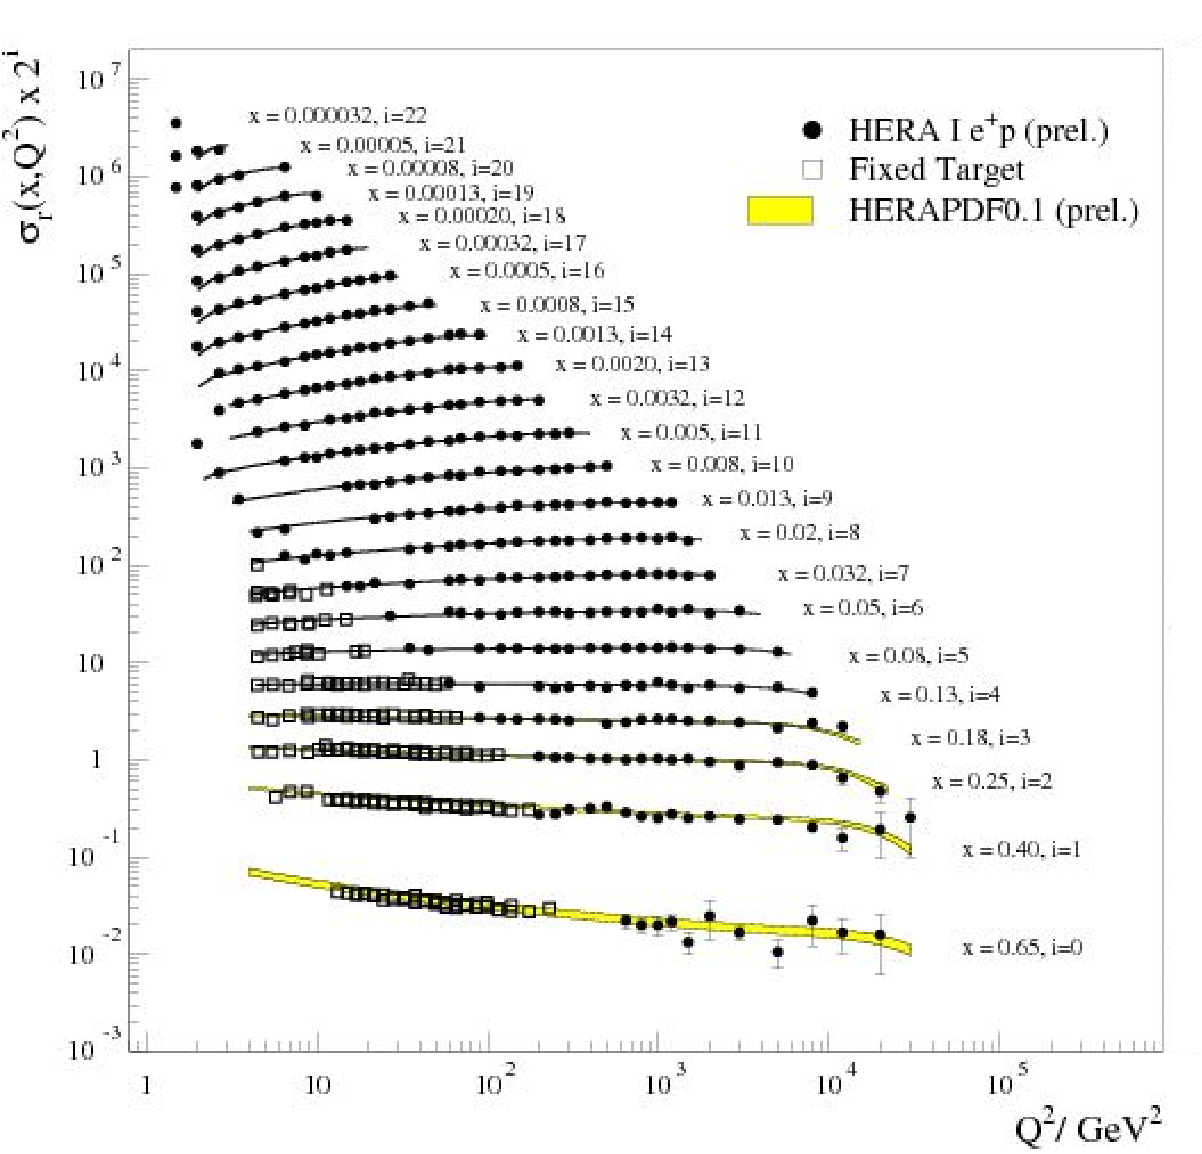
\includegraphics[scale=0.7]{HERA_PDF.pdf}
	\caption{The reduced cross section $\sigma_{r}(x,Q^2)$ as a function of $Q^2$. Filled circles are combined H1 and Zeus data from HERA for proton-positron collisions, hollow squares are from fixed target experiments, and the yellow are the $Q^2$ predictions from HERAPDF0.1.}
	\label{fig:HERA_pdf}
\end{figure}

%----------------------------------------------------------------------
%	SCIENCE GOALS SECTION
%----------------------------------------------------------------------
\section{Science Goals}
The goal of an EIC is to discover the mechanisms by which QCD is responsible for the structure and dynamics of nucleons, the nature of the nucleon-nucleon force, and the universal features of the gluon distributions at high density in the proton at low $x$.

\subsection{Nucleon Spin}
One major question still challenging nuclear physicists is ``What is the origin of the nucleon spin?''. In the 1980s the naive answer was that the total nucleon spin was the sum of the spin of its three valance quarks, but many years of experimentation has revealed that it is much more complicated (Fig. \ref{fig:nucleon_spin}), with the contributions both from quark and gluon spin and orbital angular momentum still in question. The EIC will be capable of much more detailed study of the contributions to the nucleon structure by enabling multi-dimensional projections of the distribution of quarks and gluons in space, longitudinal and transverse momenta, spin, and flavor.

\begin{figure}[!htb]
	\centering
	\includegraphics[scale=.08]{nucleon_spin.png}
	\caption{Evolution of our understanding of nucleon spin structure. Left: In the 1980s, a nucleon’s spin was naively explained by the alignment of the spins of its constituent quarks. Right: In the current picture, valence quarks, sea quarks and gluons, and their possible orbital motion are expected to contribute to overall nucleon spin. \cite{EICWhitePaper}}
	\label{fig:nucleon_spin}
\end{figure}

\subsection{The EMC Effect}
It was first observed by the European Muon Collaboration (EMC), and confirmed by other experiments that there is a modification between the nucleon structure function, $F_2$, of deuterium to those of heavier elements as a function of Bjorken $x$ \cite{SRC_EMC_effect}. Figure \ref{fig:emc_effect} shows the ratios of the Deep Inelastic Scattering (DIS) cross sections of ${}^3$He (top) to Deuterium and ${}^4$He (bottom) to Deuterium as examples of this effect. Initial assumptions were that these cross section ratios would be unity, but measurements have clearly shown a suppression in this ratio for $0.3 < x < 0.8$, the now-called EMC Effect. One can also see an enhancement of the ratio for $0.1 < x < 0.3$ known as anti-shadowing, and the region of $x < 0.1$ where the ratio is again suppressed is the shadowing region.

\begin{figure}[!htb]
	\centering
	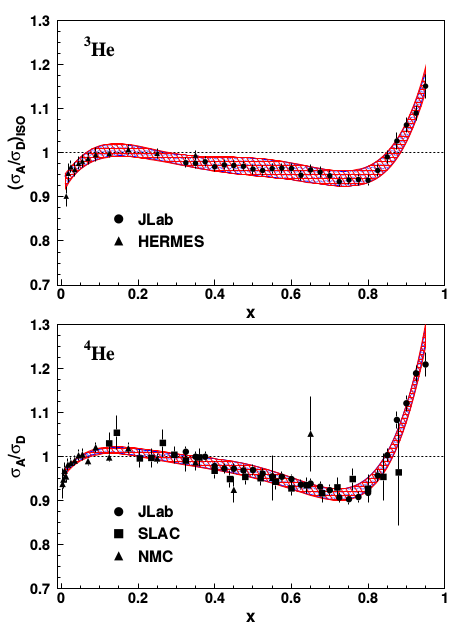
\includegraphics[scale=0.85]{EMC_He.png}
	\caption{Top: Ratios of ${}^3$He to Deuterium DIS cross sections from JLab (circles) and HERMES (triangles). Bottom: Ratios of ${}^4$He to Deuterium DIS cross sections from JLab (circles), SLAC (squares), and HERMES (triangles) \cite{EMC_Challenge}.}
	\label{fig:emc_effect}
\end{figure}

The reason for this modification to the DIS cross section is still a mystery, but the EIC hopes to shed light on this phenomenon by studying various coherent exclusive reactions, such as $J/\Psi$ production via $eA \rightarrow eAJ/\Psi$, which could allow for the quantification of initial conditions in heavy-ion collisions by mapping out the geometry of the nucleus in high-energy processes. This mapping can also help to understand other collective dynamics in inelastic collisions, such as the shadowing and anti-shadowing effects. where multiple nucleons interact coherently with the probe.

\subsection{Gluon Distributions Inside Nuclei}
As mentioned above, the EMC effect, the modification of the distribution of quarks in a nucleus versus their distribution in nucleons, is a known (yet still mysterious) phenomenon. It is suspected that this modification also occurs for gluons, with experiments such as ALICE showing evidence for gluon shadowing for $x \approx 10^{-3}$ \cite{ALICE_antishadowing}. The EIC hopes to measure this suppression of the structure functions thanks to its wider range of kinematics both in $x$ and $Q^2$, allowing not only for the measurement of gluon shadowing ($x < 0.05$), but also anti-shadowing ($x \approx 0.1$), and possibly the EMC effect for gluons ($x > 0.3$), shedding light on the origins of the EMC effect.

%----------------------------------------------------------------------
%	FACILITIES SECTION
%----------------------------------------------------------------------
\section{Facilities}
As of the writing of this thesis there are two competing designs for an EIC facility to be built in the United States: a figure-8 accelerator design for Thomas Jefferson National Accelerator Facility (JLab) (Figure \ref{fig:jleic_layout}), and a LINAC-ring (or ring-ring) accelerator design for Brookhaven National Lab (BNL) (Figure \ref{fig:erhic_layout}).

The JLab EIC (JLEIC) is planned to be approximately 1.4 km in circumference and have a footprint of roughly 500 m by 170 m. The design is a ring-ring with electrons and ions being stored in separate beam lines and collided at two interaction points  (IPs) (outlined in red in Figure \ref{fig:jleic_layout}) on the figure-8. The JLab CEBAF SRF linac will be used as an electron injector for electrons with 3 - 11 GeV/c momentum. The second ring will store an ion beam with momentum of 20 to 100 GeV/c for protons, up to 50 GeV/c per nucleon for light to medium mass N = Z nuclei, and up to 40 GeV/c per nucleon for heavy nuclei. The ion beams are generated and accelerated in a new ion injector complex with a LINAC plus figure-8 design that will be utilized to preserve ion polarization. The two main rings will be stacked vertically in the same underground tunnel \cite{JLEICdesign}.

The BNL facility, named eRHIC, will use a new electron beam facility based on an Energy Recovery LINAC that will be built inside of the Relativistic Heavy Ion Collider (RHIC) tunnel to collide with RHIC's pre-existing polarized proton/ion beam. The existing hadron ring will accelerate protons up to 250 GeV/c, $^3$He$^{+2}$ up to 167 GeV/c per nucleon, and heavier ions (e.g. gold or uranium) up to 100 GeV/c per nucleon. The new electron ring will be capable of producing electrons from 2 - 21 GeV/c \cite{eRHICdesign}. Figure \ref{fig:erhic_layout} shows the current design layout of the eRHIC facility (top) and the Brookhaven eA Solenoidal Tracker (BeAST) detector proposed for the interaction region (bottom).

%----------------------------------------------------------------------
%	PARTICLE ID SUBSECTION
%----------------------------------------------------------------------
\subsection{Particle Identification Requirements and Solutions}
The large center of mass energies and diverse physics program at an EIC necessitate a very sophisticated detector suite. The most basic process that the EIC will observe is inclusive DIS with nearly full reconstruction of the hadronic final state. The ability to accurately identify hadrons in the final state is therefore a key requirement for the physics program, as is shown by Figure \ref{fig:pythia_DIS} which shows the momentum distributions of pions and kaons for each region of interest for typical beam energies for both BNL and JLab.

As can be seen in Figures \ref{fig:jleic_layout} and \ref{fig:erhic_layout}, the layouts of the two detector concepts for JLab and BNL are slightly different, but the solutions for PID requirements are very similar. In the hadron endcap, because of the large final state energies the ideal PID detector would be a gaseous, mirror-based Ring Imaging Cherenkov (RICH) detector. This will provide $\pi/K/p$ separation up to 50 GeV/c momentum. The hadrons produced going towards the electron endcap scales in both energy and quantity with the energy of the electron beam energy. Although the maximum electron beam energies of JLab and BNL differ, PID up to 10 GeV/c momentum seems to be suitable for both facilities, and so a modular aerogel RICH detector is currently under development. In the central barrel region the necessary momentum coverage is not as high as that of the endcaps because the transverse momentum transfer from the electron beam to the ion beam is generally less than 10 GeV/c. This smaller momentum range coupled with a smaller space to fit a detector make a detector based on Detection of Internally Reflected Cherenkov light (DIRC) technology a desirable choice.

The design and prototype testing of components for a high-performance DIRC detector is the subject of this thesis and an ideal solution for PID in the EIC barrel region.


\begin{figure}[!htb]
	\centering
	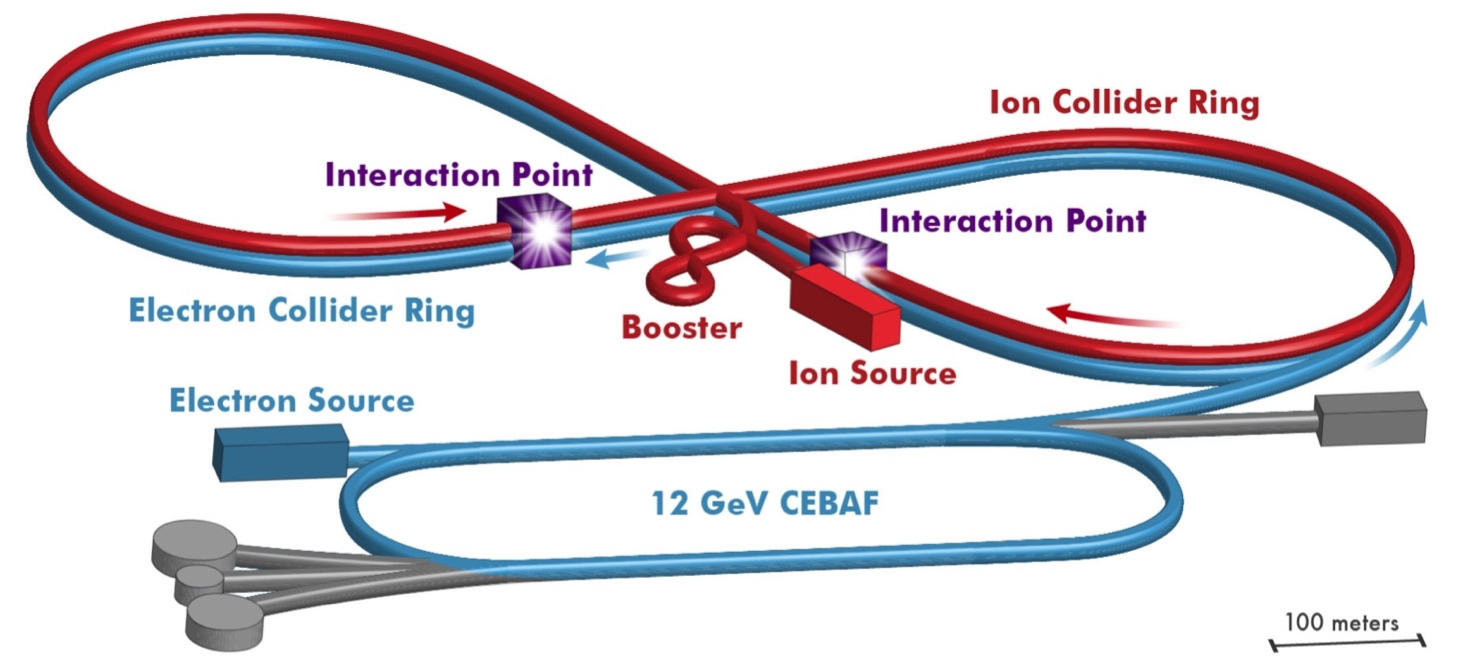
\includegraphics[width=\textwidth]{JLEIC_layout3.jpg}
	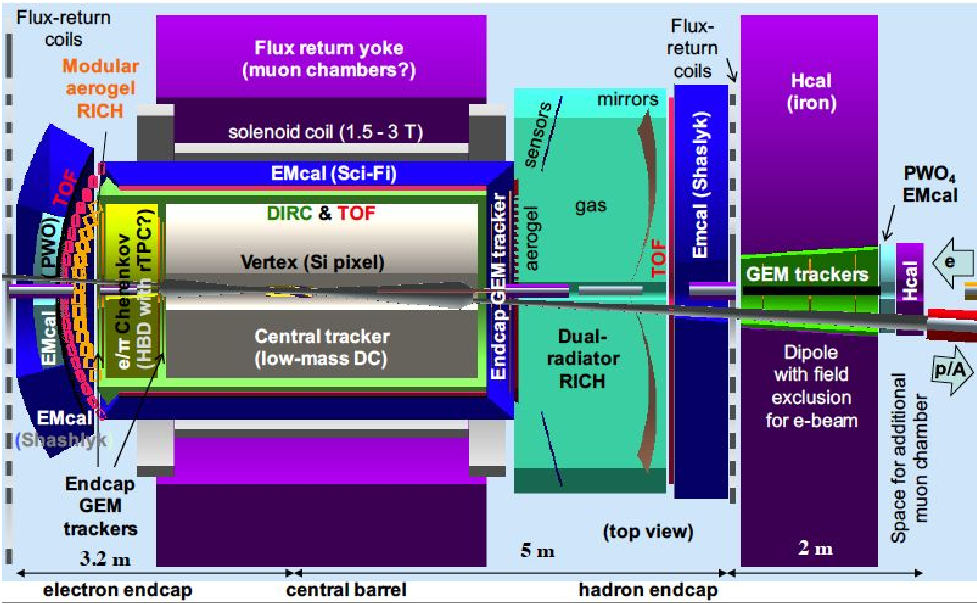
\includegraphics[width=\textwidth]{JLEIC_detector.pdf}
	\caption{A design of the EIC facility for JLab with the two interaction points (IP) highlighted in purple (top), and the current baseline design for the detector at the left-most IP. (bottom).}
	\label{fig:jleic_layout}
\end{figure}

\begin{figure}[!htb]
	\centering
	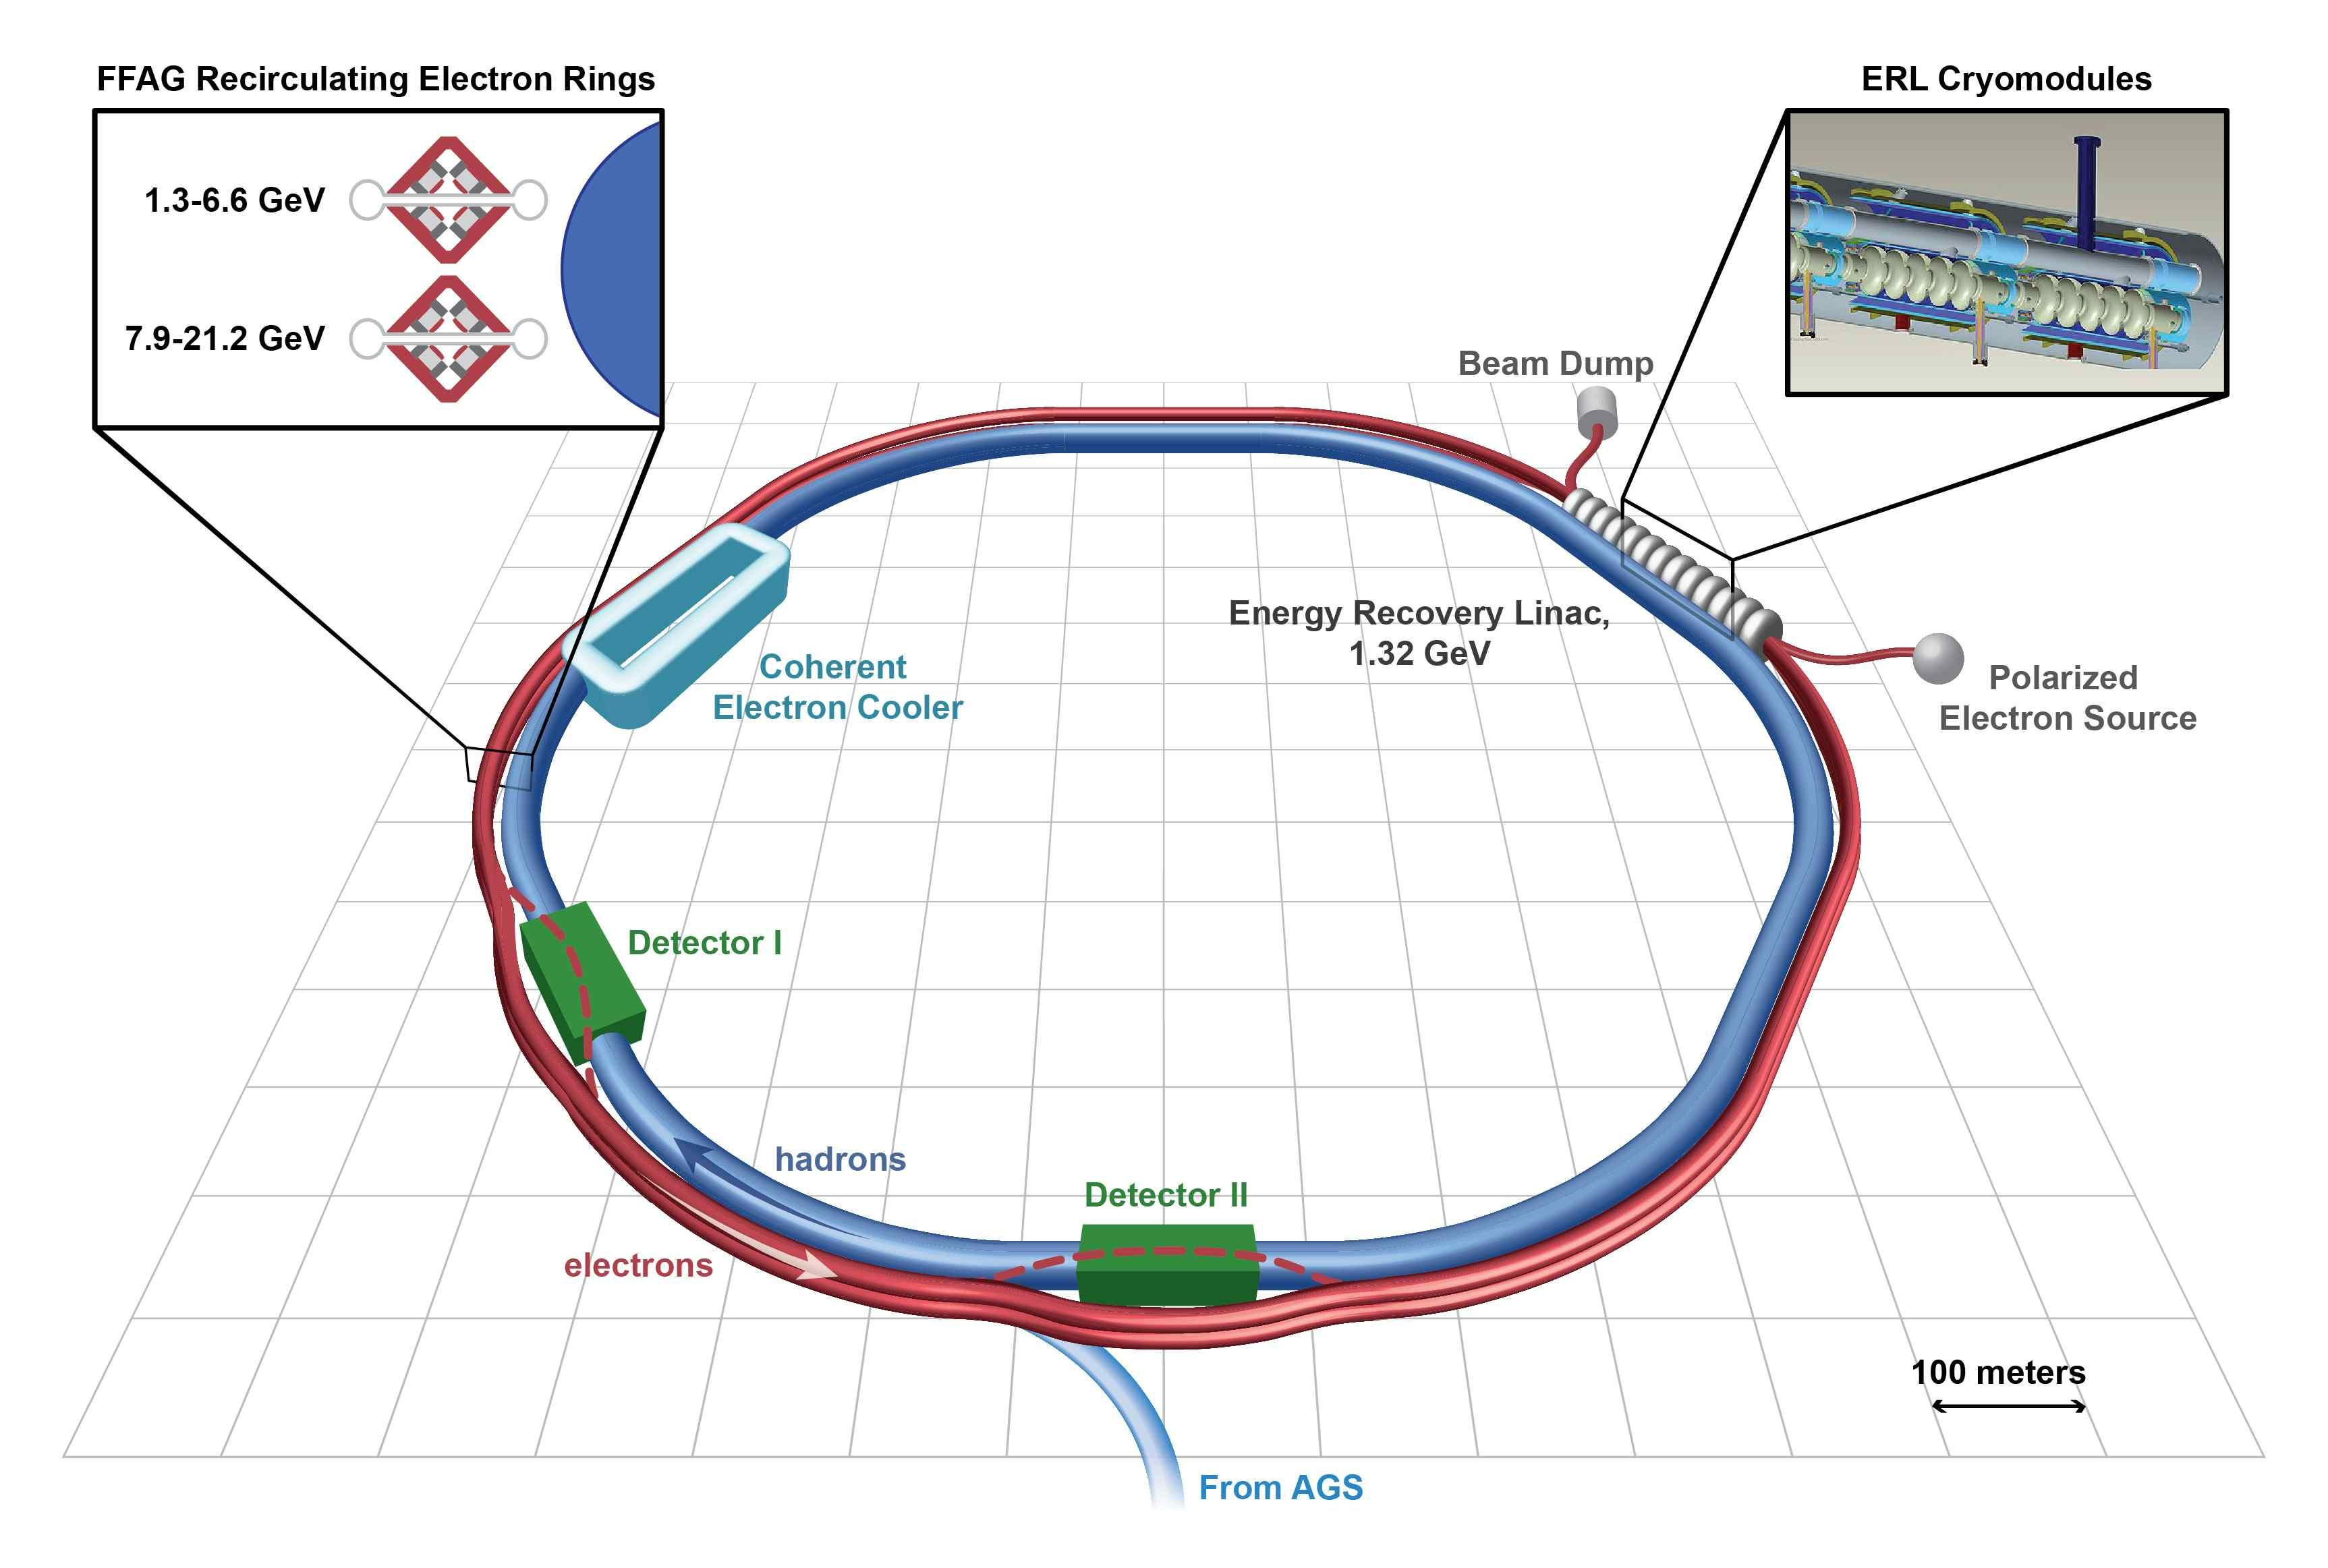
\includegraphics[width=\textwidth]{eRHIC_Layout.jpeg}
	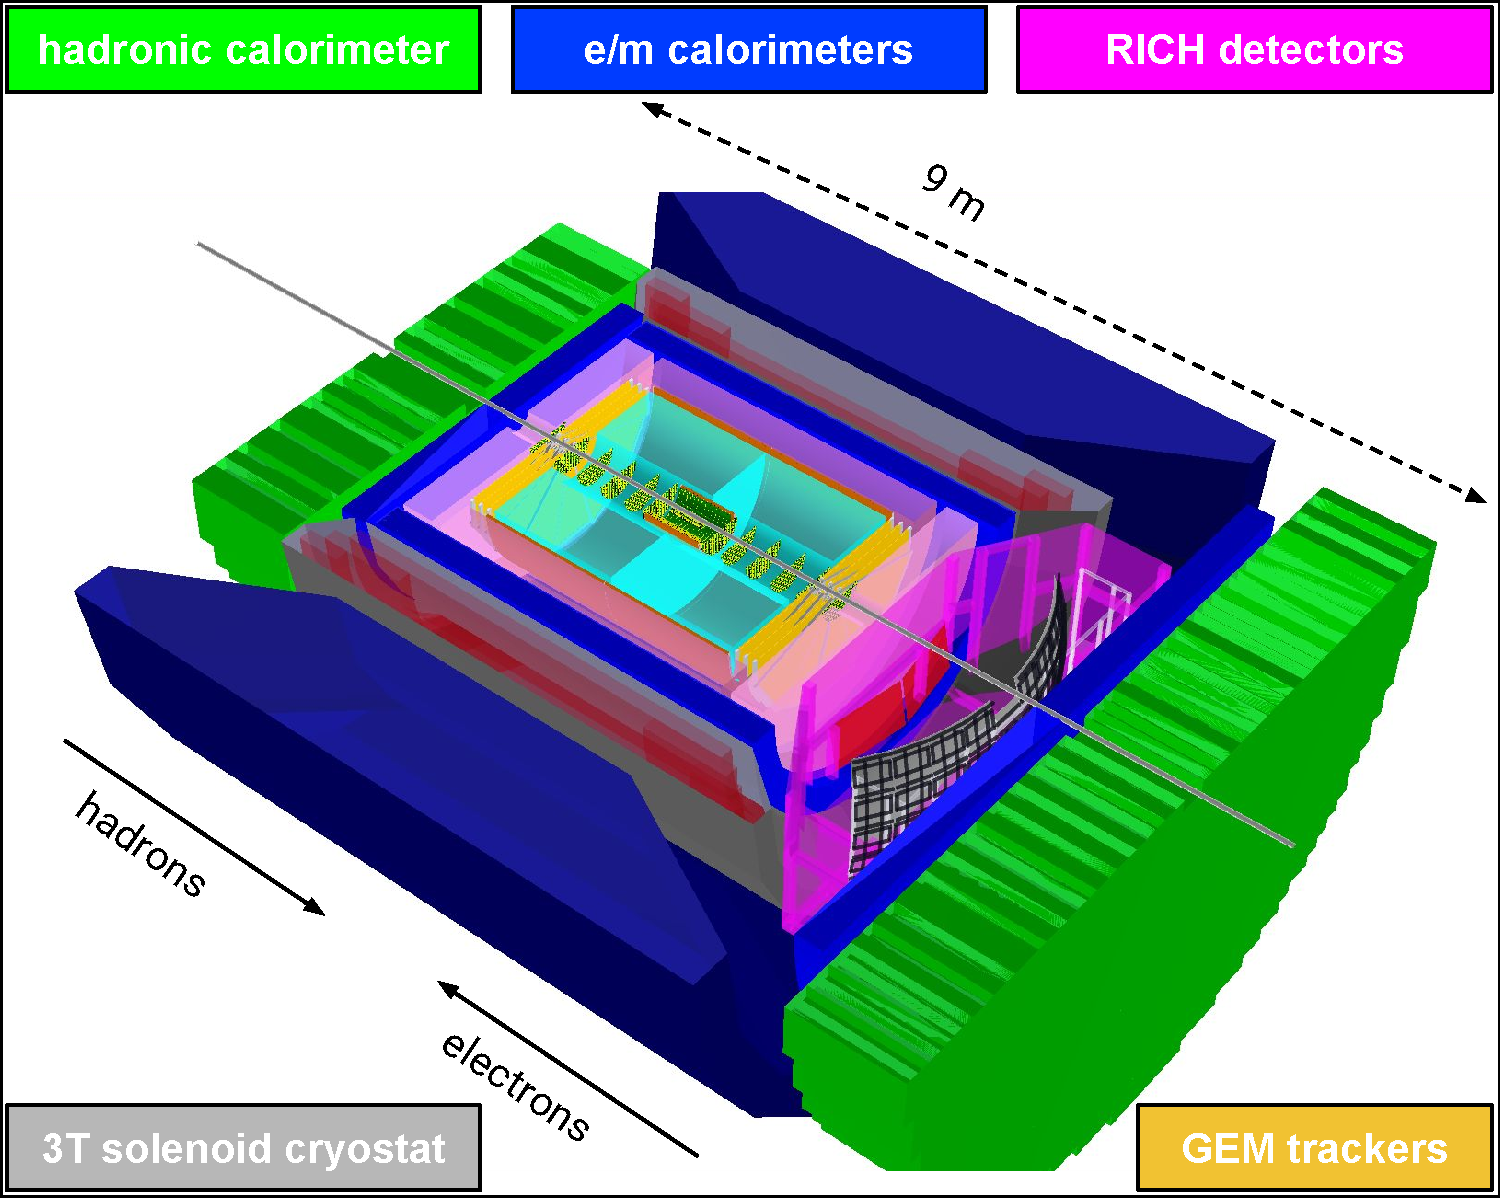
\includegraphics[width=0.9\textwidth]{eRHIC_beast.pdf}
	\caption{A design of the LINAC-ring option for an EIC facility at BNL (top), and the proposed BeAST (Brookhaven eA Solenoidal Tracker) detector (bottom).}
	\label{fig:erhic_layout}
\end{figure}

\begin{figure}[!htb]
	\centering
	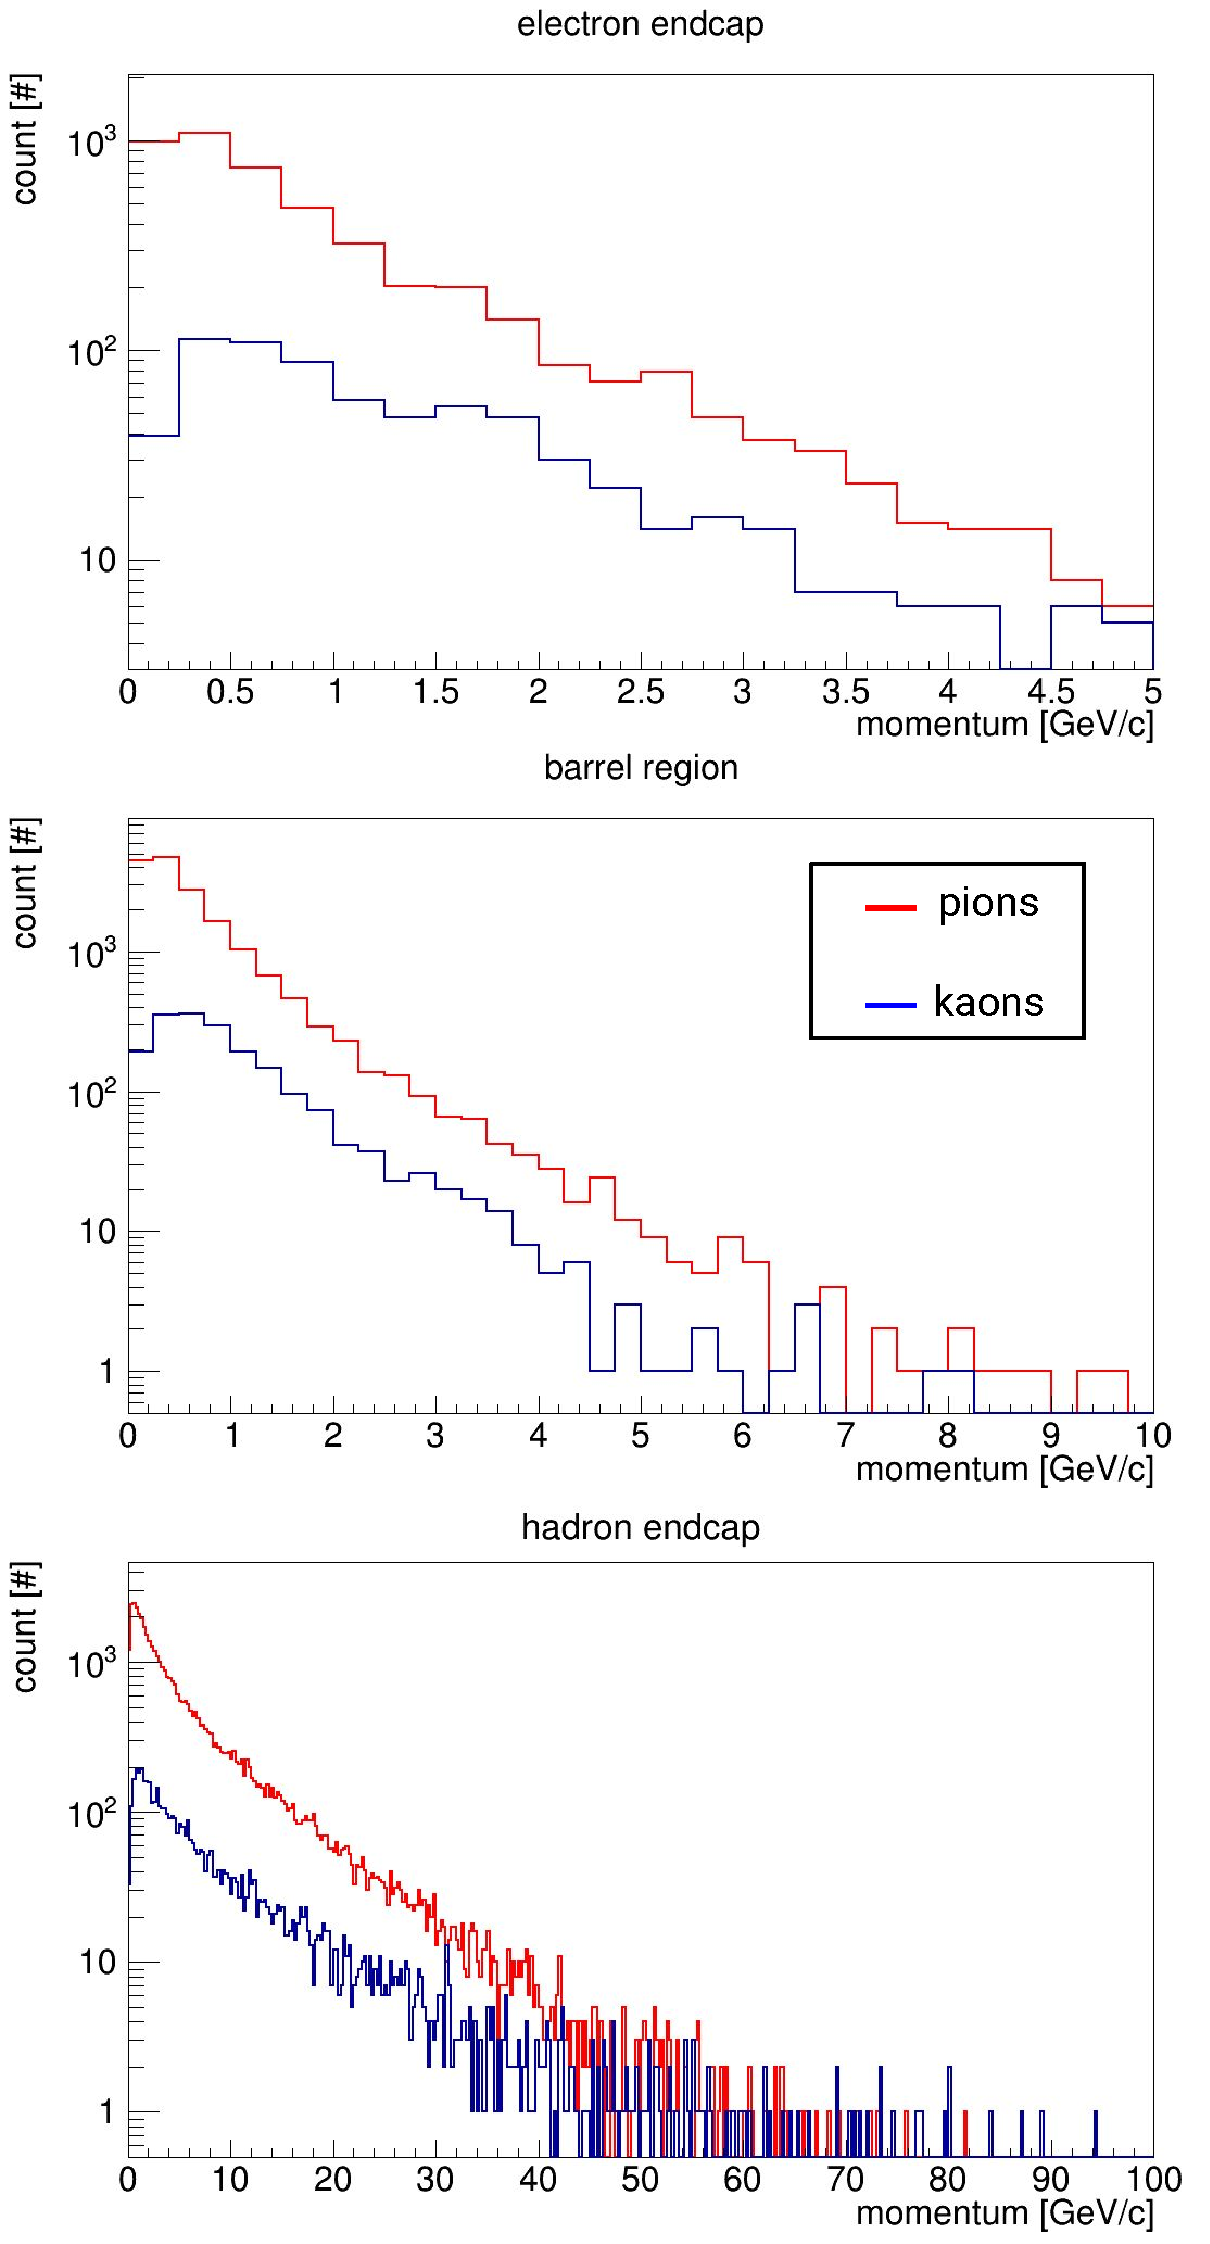
\includegraphics[width=0.72\textwidth]{pythia_DIS_regions.pdf}
	\caption{Momentum distributions for pions (red) and kaons (blue) in the electron endcap (top), barrel region (middle), and hadron endcap (bottom). Plots were produced using the pythia simulation package for DIS events corresponding to collisions between 10 GeV electrons and 100 GeV protons, a common BNL/JLab kinematic, shown for a bin of $10<Q2<100\unit{GeV}^2$.}
	\label{fig:pythia_DIS}
\end{figure}
